\documentclass{article}
\usepackage[utf8]{inputenc}
\usepackage{graphicx}
\usepackage[portuguese]{babel}
\usepackage{float}
\usepackage{xcolor}
\title{Trabalho em Grupo}
\author{Fran Adalid Cardoso Alvarez e Paloma Zankely Alves de Oliveira Cione}
\date{Novembro de 2019}

\begin{document}

\maketitle

\section{Referencial teórico}
\subsection{Certificação digital}
Certificado digital é um arquivo eletrônico que serve como identidade virtual para uma pessoa física ou jurídica, e por ele pode-se fazer transações online com garantia de autenticidade e com toda proteção das informações trocadas.

Um certificado digital é usado para ligar uma entidade a uma chave pública. No caso de uma Infraestrutura de Chaves Públicas (ICP), o certificado é assinado pela Autoridade Certificadora (AC) que o emitiu, e no caso de um modelo de Teia de Confiança (Web of trust), como o PGP, o certificado é assinado pela própria entidade e assinado por outros que dizem confiar naquela entidade. Em ambos os casos as assinaturas contidas em um certificado são atestamentos feitos por uma entidade que diz confiar nos dados contidos naquele certificado. 
Um certificado normalmente inclui:
\begin{itemize}
\item{Informações referentes à entidade para o qual o certificado foi emitido (nome, email, CPF/CNPJ, PIS etc.).}
\item{A chave pública referente a chave privada de posse da entidade especificada no certificado.}
\item{O período de validade.}
\item{A localização do "centro de revogação" (uma URL para download da LCR, ou local para uma consulta OCSP).}
\item{A(s) assinatura(s) da(s) AC/entidade(s) que afirma que a chave pública contida naquele certificado confere com as informações contidas no mesmo.}
\end{itemize}
\subsection{SSL/TLS}
O objetivo do SSL/TLS é tornar segura a transmissão de informações sensíveis como dados pessoais, de pagamento ou de login. É possível identificar que um site possui certificado SSL/TLS quando há um cadeado indicando a conexão segura próximo à URL no navegador.

\textbf{SSL} significa Secure Sockets Layer, um tipo de segurança digital que permite a comunicação criptografada entre um site e um navegador. Atualmente a tecnologia se encontra depreciada e está sendo completamente substituída pelo TLS.

\textbf{TLS} é uma sigla que representa Transport Layer Security e certifica a proteção de dados de maneira semelhante ao SSL. Como o SSL não está mais de fato em uso, esse é o termo correto que deveria ser utilizado.

O SSL/TLS funciona através de chaves públicas e privadas, além de chaves de sessão para cada conexão segura. Quando o visitante coloca uma URL com SSL/TLS no navegador e navega pela página segura, o navegador e o servidor fazem uma conexão.

Durante a conexão inicial as chaves públicas e privadas são utilizadas para criar uma chave de sessão, que então é utilizada para criptografar e descriptografar os dados sendo transferidos. Essa chave de sessão vai se manter válida por tempo limitado e só vai ser utilizada para essa sessão específica.

\begin{figure}[h]
\centering
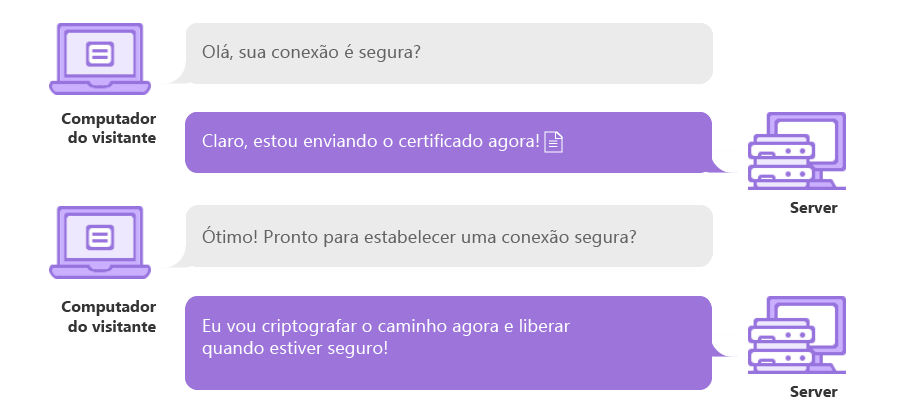
\includegraphics[width=13.5cm]{imagem1.png}
\caption{Exemplo de conexão SSL/TLS}
\end{figure}
\subsection{Projeto Let’s Encrypt}
Let's Encrypt é uma autoridade certificadora não-lucrativa comandada pelo "Internet Security Research Group (ISRG)" que fornece certificados \textbf{X.509} (formato padrão de certificados de chaves públicas) para TLS gratuitamente. O certificado é válido por 90 dias, o qual pode ser renovado a qualquer momento. Os certificados são criados através de um processo automatizado, feito  para eliminar a complexidade dos processos atuais de criação, validação, instalação e renovação de certificados para sites seguros.

O projeto busca tornar as conexões criptografadas ubíquas para todos os servidores da World Wide Web. Ao eliminar barreiras como pagamento, e a renovação do certificado, espera-se diminuir significativamente a complexidade de configurar e manter criptografia TSL.
\subsection{Protocolo ACME}
O protocolo ACME (Automatic Certificate Management Environment) foi projetado pelo ISRG para seu projeto "Lets Encrypt". É um protocolo de comunicação feito para automatizar interações entre autoridades certificadoras e os servidores web de seus usuários, permitindo o desenvolvimento automatizado de uma infraestrutura de chaves públicas de forma que haja um custo baixo. 

\end{document}

